 % \documentclass[a4paper, draft]{report}
\documentclass[a4paper, 10pt]{report}


\usepackage[utf8]{inputenc}
\usepackage[T1]{fontenc}
\usepackage[margin=2.5cm]{geometry}
\usepackage{csquotes}
\usepackage{hyphenat}
\usepackage{biblatex}
\usepackage{graphicx}
\usepackage{float}
\usepackage{caption}
\usepackage{subfig}
\usepackage{textcomp}
\usepackage{gensymb}
\usepackage{booktabs}
\PassOptionsToPackage{hyphens}{url}\usepackage{hyperref}
\usepackage{listings}
\usepackage{lmodern}
\usepackage{amsmath}
\usepackage{amssymb}
\usepackage{siunitx}
\usepackage{enumitem}
\usepackage[acronym]{glossaries}
\usepackage{tabularx}
\usepackage{xltabular}
\usepackage{setspace}
\usepackage{tablefootnote}


\usepackage{tablefootnote}

% \usepackage[scale=1.0]{draftwatermark}

\addbibresource{biblio.bib}
\newacronym{ad}{AD}{Algorithmic/Automatic Differentiation}
\newacronym{sa}{SA}{Spalart Allmaras}
\newacronym{imes}{IMES}{Institute for mechanical systems}

\graphicspath{
    {img}
    {fundamentals/img}
    {methods/img}
    {results/img}
}
% \hyphenation{Mathe-matik wieder-gewinnen}

% use 1e-10 instead of 1 x 10^(-10)
\sisetup{output-exponent-marker=\ensuremath{\mathrm{e}}}



% \title{Adaption of the SST turbulence model for optimization in ADflow}
% \author{David Anderegg}

% Add Numbering to chapters
\makeatletter
\def\@makechapterhead#1{%
  \vspace*{50\p@}%
  {\parindent \z@ \raggedright \normalfont
    \interlinepenalty\@M
    \Huge\bfseries  \thechapter.\quad #1\par\nobreak
    \vskip 40\p@
  }}
\makeatother

\renewcommand{\arraystretch}{1.1}



\usepackage{fancyhdr}
\setlength{\headheight}{34pt}

\renewcommand{\headrulewidth}{0.5pt}
\renewcommand{\footrulewidth}{0.5pt}


\fancypagestyle{plain}{
    % header inputs
    \lhead{IMES}
    \chead{Adaption of the SST turbulence model for optimization in ADflow}
    \rhead{
\includegraphics[width=1cm]{uni_header}}


    %footer inputs
    % \lfoot{Innosuisse 35172.1 IP-ENG}
    \cfoot{Page  \thepage}
    \rfoot{\today}
}
\pagestyle{plain}

\setlength{\parskip}{.25em}

\begin{document}
    \begin{titlepage}

    % Defines a new command for the horizontal lines, change thickness here
    \newcommand{\HRule}{\rule{\linewidth}{0.5mm}} 

    \center % Center everything on the page

    %--------------------------------------------------------------------------
    %   HEADING SECTIONS
    %--------------------------------------------------------------------------

    % Name of your university/college
    \textsc{\LARGE Zurich University of Applied Sciences}\\[1.5cm] 
    % Major heading such as course name
    \textsc{\Large Specialization Project 2}\\[0.5cm] 
    % Minor heading such as course title
    \textsc{\large Institute of Mechanical Systems}\\[0.5cm] 

    %--------------------------------------------------------------------------
    %   TITLE SECTION
    %--------------------------------------------------------------------------

    \HRule 
    { \huge \bfseries
    \begin{spacing}{1.2}
        Adaption of the SST turbulence model for optimization in ADflow
    \end{spacing}}
    \HRule \\[0.5cm]

    %--------------------------------------------------------------------------
    % AUTHOR SECTION
    %--------------------------------------------------------------------------

    \begin{minipage}{0.4\textwidth}
        \begin{flushleft} \large
            \emph{Author:}\\
            David Anderegg\\
            %\secondauthorfirstname \textsc{\secondauthorlastname}% Your name
        \end{flushleft}
    \end{minipage}
    ~
    \begin{minipage}{0.4\textwidth}
        \begin{flushright} \large
            \emph{Supervisor:} \\
            Prof. Marcello Righi \\
            Dr. Anil Yildirim (Michigan)
        \end{flushright}
    \end{minipage}\\[1.5cm]

    % If you don't want a supervisor, uncomment the two lines below and remove
    % the section above
    %\Large \emph{Author:}\\
    %John \textsc{Smith}\\[3cm] % Your name

    %--------------------------------------------------------------------------
    % DATE SECTION
    %--------------------------------------------------------------------------

    % Date, change the \today to a set date if you want to be precise
    {\large \today}\\[2cm] 

    %--------------------------------------------------------------------------
    % LOGO SECTION
    %--------------------------------------------------------------------------

     % Include a department/university logo
    
\includegraphics[width=0.5\textwidth]{img/en-zhaw-imes-sw.png}\\[2cm]


    %--------------------------------------------------------------------------

    \vfill % Fill the rest of the page with whitespace
    % \pagenumbering{alph}

\end{titlepage}



    \begin{abstract}

        With the increase of available computer power, Reynolds Averaged Navier
        Stokes (RANS) based optimizations become more and more viable. For
        conventional flow analysis, the correct turbulence model is
        detrimental to obtain correct results. This dependence may be even
        exaggerated for optimizations as the turbulence model is responsible
        for various aerodynamic effects the optimizer might exploit.

        This work extends the number of available turbulence models in the open
        source CFD solver ADflow by adding the \textit{menter SST} model.
        ADflow is specialized in optimizations and uses the \textit{adjoint
        method} to compute the gradients needed in an efficient manner. To make
        the SST available for optimizations, the changes have been
        differentiated using Automatic Differentiation (AD). 

        The implemented model is verified by comparing the results of the "2D
        bump" testcase to reference data. The partial and total gradients are
        verified using finite differences, complex step and the dot-product
        test. 

        The results show that SST is most likely implemented correctly. Also
        the Newton type solvers available in ADflow seem to work with SST. But
        the obtained total gradients are only partially correct. To summarize,
        this project provides a prototype implementation which still needs some
        time to iron out the remaining bugs.
    \end{abstract}

    \tableofcontents\clearpage


    \chapter{Introduction}
    High fidelity optimization using gradient based approaches have become more and
more popular. This may be explained through the fact that they do not suffer
from the \textit{curse of dimensionality}. This allows them to have a much
higher number of design variables (dvs) compared to alternatives such as genetic
optimization approaches. The drawback is, of course, one must compute the
gradients in an efficient manner. The \textit{MACH-Aero} Framework offers a set
of tools for gradient based high-fidelity optimization. Part of this Framework
is a CFD solver called \textit{ADflow} which has only one working turbulence
model. This project aims to change that through the implementation of the $k$ -
$\omega$ \textit{Shear Stress Transport (SST)} model.








\section{ADflow}
ADflow is an open-source multi-block\footnote{Overset meshes are also
possible.} Computational Fluid Dynamics (CFD) solver. It solves the Reynolds
Averaged Navier Stokes (RANS) equations to obtain the flow solution. It is
developed and maintained at the \textit{MDOLab} at the university of Michigan
and was based on a CFD solver for turbo machinery called \textit{sumb}. It has
later been adopted  for gradient based optimization by means of
\textit{Algorithmic Differentiation}\footnote{Thats what AD stands for in
ADflow.} and the \textit{adjoint method}. Most of ADflow is written in Fortran.
But it is interfaced in Python. This means, the heavy lifting is done in a fast
language, but the regular user has the benefits of an object-oriented high
level interpreter language.
 
In optimization, a lot of simulations are necessary until an optimal design is
found. It is also highly important to always get an objective value for each
design, even if, or especially when, it is unphysical. Otherwise the optimizer
does not know how bad the current design is. To cater those concerns, ADflow
employs some highly efficient and robust NK\footnote{NK stands for the
Newton–Krylov method.} and ANK\footnote{ANK is an approximated Newton–Krylov
method.} solvers. Those can achieve machine-precision convergence, even for
aircraft configurations at an angle of attack of 90\degree \cite{Mader2020a}
\cite{Kenway2019a} \cite{Yildirim2019b}.

When the solver was still called sumb, various turbulence models such as
Spalart-Allmaras, Spalart-Allmaras with Edwards Modification, $k$ - $\omega$
Wilox, $k$ - $\omega$ Wilox modified, $k$ - $\tau$, v2-f and Menter SST were
implemented. The subsequent modification for optimizations changed the
structure dramatically and only the SA model was carried over. But this means,
a skeleton implementation of SST is available and only the structural changes
need to be incorporated.


\section{Goals}
As stated above, the legacy code for SST is still available but does not really
work anymore. The goal for this project is to get it working for simulation and
optimization. The necessary sub-steps may be summarized as follows. Please note
some in-depth knowledge is needed to understand them. But this will be
explained in later sections of this report:

\begin{enumerate}
    \item Get the current SST model running using a legacy DADI-method.

    \item Modify it in such a way that it is automatically differentiate-able.

    \item Actually differentiate it through \textit{Automatic/Algorithmic
        Differentiation (AD)}.

    \item Make sure the partial AD derivatives are correct. 

    \item Get the NK/ANK Solver working.

    \item Test and verify the implementation

    \item Get the adjoint Solver working.

    \item Test and verify the total gradients.
\end{enumerate}








\section{Code contributions}
Part of this project is a code contribution to ADflow and a setup of test
cases, both can be found on GitHub under those links:\\

\begin{tabular}{l l}
    ADflow Pull Request &
    \url{https://github.com/mdolab/adflow/pull/301}\footnotemark \\

    Test cases & \url{https://github.com/DavidAnderegg/SST_rough_testcases}
\end{tabular}


\footnotetext{The commit at the time of writing was: \texttt{361bf3e9a2e1e4fee177becfdc94f1e48809fa2e}}


    \chapter{Theoretical Fundamentals}
    \section{Reynold's Averaged Navier Stokes (RANS).}
The \textit{Navier-Stokes} equations establish the connection between the
velocity ($U$), pressure ($P$), temperature ($T$), and density ($\rho$) of a
moving fluid. These equations, represented as partial differential equations,
are typically challenging to solve analytically. Consequently, numerical
methods become necessary. The physical properties are functions of four
variables: spatial coordinates (x, y, z), and time (t). To apply numerical
methods effectively, these properties must be discretized \cite{nasaNS}.

In flows with high Reynolds numbers, various eddies have significantly
different length and time scales. Properly capturing the smallest eddies,
essentially representing turbulence, would require an extremely fine mesh and
time step, rendering it impractical. To address this challenge, simplifications
are necessary: (1) considering a steady flow instead of unsteady, and (2)
accounting for turbulence in a stochastic manner. By adopting these approaches,
a single simulation (instead of one every x milliseconds) and a coarser grid
become sufficient to achieve meaningful results.


\subsubsection{Reynolds averaging}
In 1895, Osborne Reynolds introduced a solution that would later be referred to
as \textit{Reynolds Averaged Navier-Stokes}. The fundamental concept involves
dividing the velocity (along with other resolved physical properties) into two
components\cite{leschziner2015statistical} :

\begin{equation}
    U_{i} = \bar U_{i} + u_{i}^{\prime} \qquad
    P = \bar P + p^{\prime}
\end{equation}

\noindent The subscript $i$ represents all three spatial coordinates (x, y, z).
The mean velocity, denoted as $\bar U_{i}$, remains constant, while
$u_{i}^{\prime}$ represents the fluctuating component caused by turbulence,
which remains unresolved. The same notation applies to the pressure $P$.
Substituting these expressions into the incompressible Navier-Stokes equations
results in:

\begin{equation}
    \label{eq:incomp_RANS}
    \frac{\partial \rho \bar U_{i} \bar U_{j}}{\partial x_{j}} =
    \frac{\partial \bar P}{\partial x_{i}} +
    \frac{\partial}{\partial x_{j}} \nu (\frac{\partial 
    \bar U_{i}}{\partial x_{j}} +
    \frac{\partial \bar U_{j}}{\partial x_{i}}) -
    \frac{\partial}{\partial x_{j}} \rho u_{i}^{\prime} u_{j}^{\prime}
\end{equation}

\noindent The \textit{six} independent \textit{Reynolds-stresses} are
represented by $\rho u_{i}^{\prime} u_{j}^{\prime}$. It is important to note
that the fluctuating component for pressure, $p^{\prime}$, cancels out and does
not reappear. The Reynolds stresses can be denoted using tensor notation:

\begin{equation}
    \rho \bar u_{i} \bar u_{j} = \rho
    \begin{pmatrix}
        u_{1}^{\prime 2}              & u_{1}^{\prime} u_{2}^{\prime} & 
        u_{1}^{\prime} u_{3}^{\prime} \\

        u_{2}^{\prime} u_{1}^{\prime} & u_{2}^{\prime 2}              & 
        u_{2}^{\prime} u_{3}^{\prime} \\

        u_{3}^{\prime} u_{1}^{\prime} & u_{3}^{\prime} u_{2}^{\prime} & 
        u_{3}^{\prime 2}
    \end{pmatrix}
\end{equation}

\noindent Equation \ref{eq:incomp_RANS} is complemented by the Reynolds-averaged
mass-conservation equation:

\begin{equation}
    \frac{\partial \rho \bar U_{j}}{\partial x_{j}} = 0
\end{equation}


\subsubsection{Turbulence model}
To determine the unknown Reynolds stresses, a \textit{turbulence model} is
employed. Among several approaches, the two most commonly used are \textit{Eddy
viscosity} models and \textit{Reynolds stress transport} models. The SST model
belongs to the former category, and therefore, it will be elaborated on in more
detail.


\paragraph{Eddy viscosity models}
These kind of models depend on the \textit{Boussinesq-assumption} which says
that the effect of turbulence is similar to that of an increased viscosity.
Thus, it introduces the \textit{eddy viscosity} $\mu_{t}$. After some equation
mangling one may calculate the Reynolds stresses from the eddy viscosity as
follows:

\begin{equation}
    - \rho u_{i}^{\prime} u_{j}^{\prime} =
    \nu_{t} (\frac{\partial \bar U_{i}}{\partial x_{j}} +
    \frac{\partial \bar U_{j}}{\partial x_{i}}) -
    \frac{2}{3} \delta_{ij} \rho k
    \label{eq:boussinesq}
\end{equation}

\noindent Where

\begin{align*}
    \delta_{ij} = \; &0 \qquad \text{for} \qquad i \neq j \\
    &1 \qquad \text{for} \qquad i = j
\end{align*}

\noindent and $k$ is the \textit{turbulent kinetic energy}. Thus the calculation
of the six Reynolds-stresses has reduced to calculating $\nu_{t}$ and $k$
\cite{leschziner2015statistical}.




\subsection{$k$ - $\epsilon$ model}




\subsection{$k$ - $\omega$ model}




\subsection{$k$ - $\omega$ SST model}




    \chapter{Methods}
    methods



    \chapter{Results}
    \section{Solver Convergence}
\subsubsection{NACA0012}
Figure \ref{fig:sc_NACA0012} shows the solver convergence for the NACA0012
testcase. The baseline implementation and the final state when writing this
report (modified) is shown. Both states were run once with 1 and 6 cpus.

\begin{figure}[H] \centering
    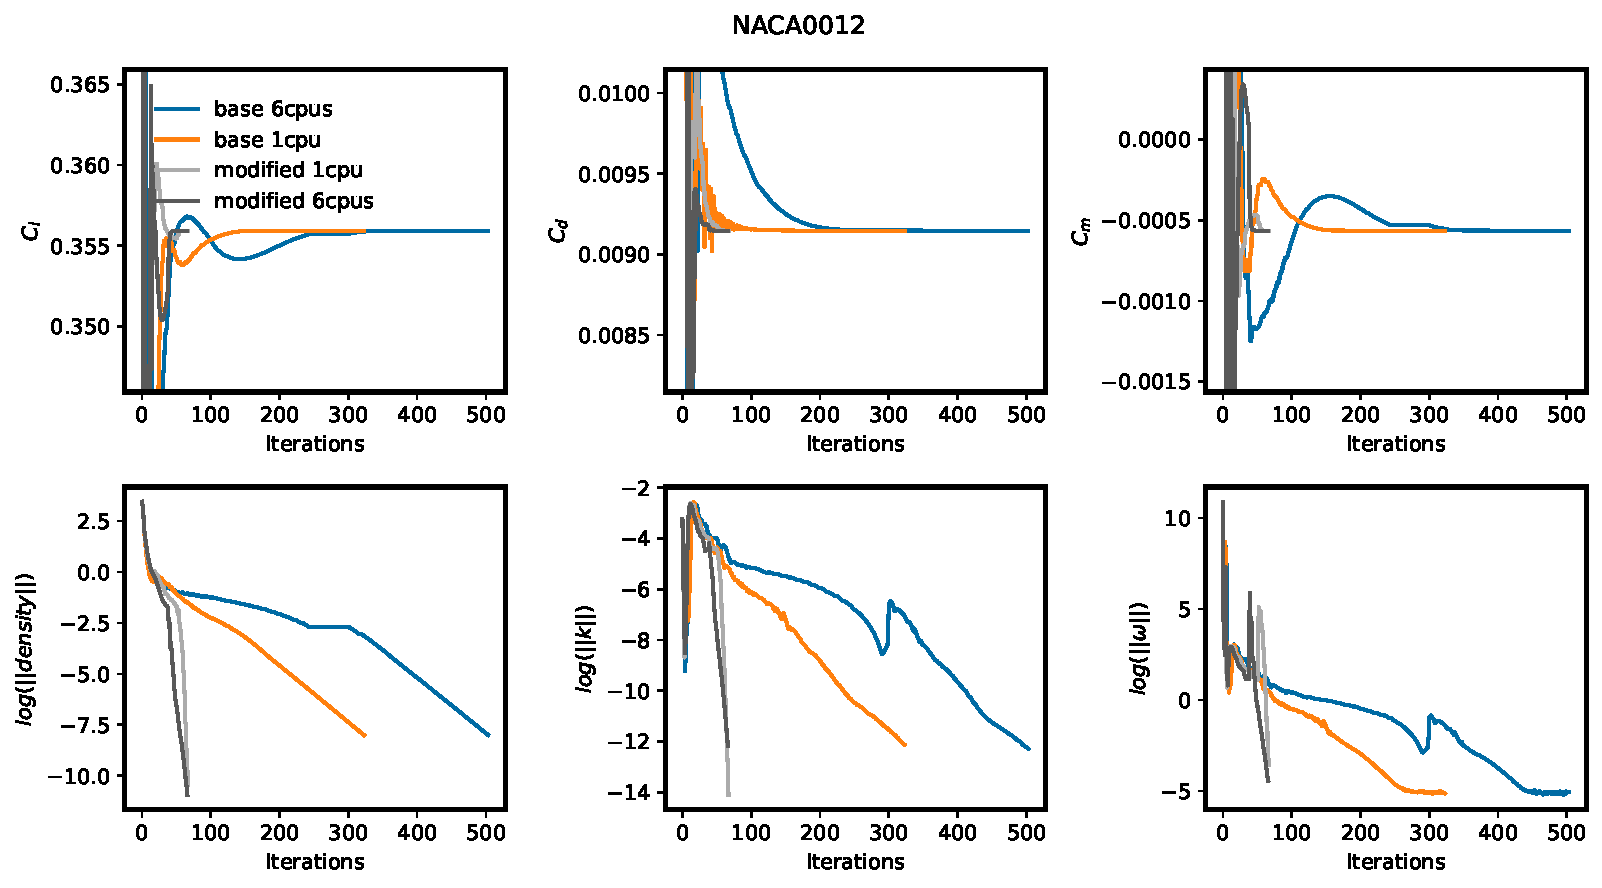
\includegraphics[width=1.0\textwidth]{plots/sc_NACA0012}
    \caption{Convergence history for NACA0012 testcase.}
    \label{fig:sc_NACA0012}
\end{figure}

\noindent Lets take a look at the baseline implementation first. It was
obtained using the ANK solver and a decoupled DADI solver for the turbulence
model. For the turbulence model, a total of 20 sub iterations were used. When
looking at the functions values (top row), it can be seen that 1 and 6 cpus
reach the same value. But 6 cpus need more iterations. It is not quite clear
what causes this, but it is a known phenomenon for low cpu counts and vanishes
when this number is increased. Production runs usually require tens or even
hundrets of cpus and thus this is not considered detrimental.


Now, lets look at the modified curves. Here, SST was differentiated and the
turbulence ANK and fully coupled CANK solvers are available. Annectdotal
evidence suggest SST is highly non-linear. This is especially true for the
inital stages of convergence. Due to this\footnote{The author believes the ANK
solver does some finite-differencing for some terms under the hood.}, the
turbulence DADI solver is way more efficient early on. Thus, at the beginning,
the regular ANK solver with decoupled DADI was used. But once a relative
convergence of 1e-6 is reached, the second order coupled ANK (CSANK) is
engaged. Once it gets traction, it exhibits almost Newton-like convergence. The
number of cpus does not really affect the number of iterations needed. It is
also obvious that the modified version approaches the same function values as
the baseline implementation. 




\subsubsection{RAE2822}
Figure \ref{fig:sc_RAE2822} shows a similar convergence plot for the RAE2822
testcase. Once again, the baseline and modified version with each 1 and 6 cpus
is plotted. It is important to note that this case is somewhat hard as it lies
in the transsonic regimes where shocks appear. But at the same time, it is even
coarser than the naca case which makes it hard to resolve them properly.

\begin{figure}[H] \centering
    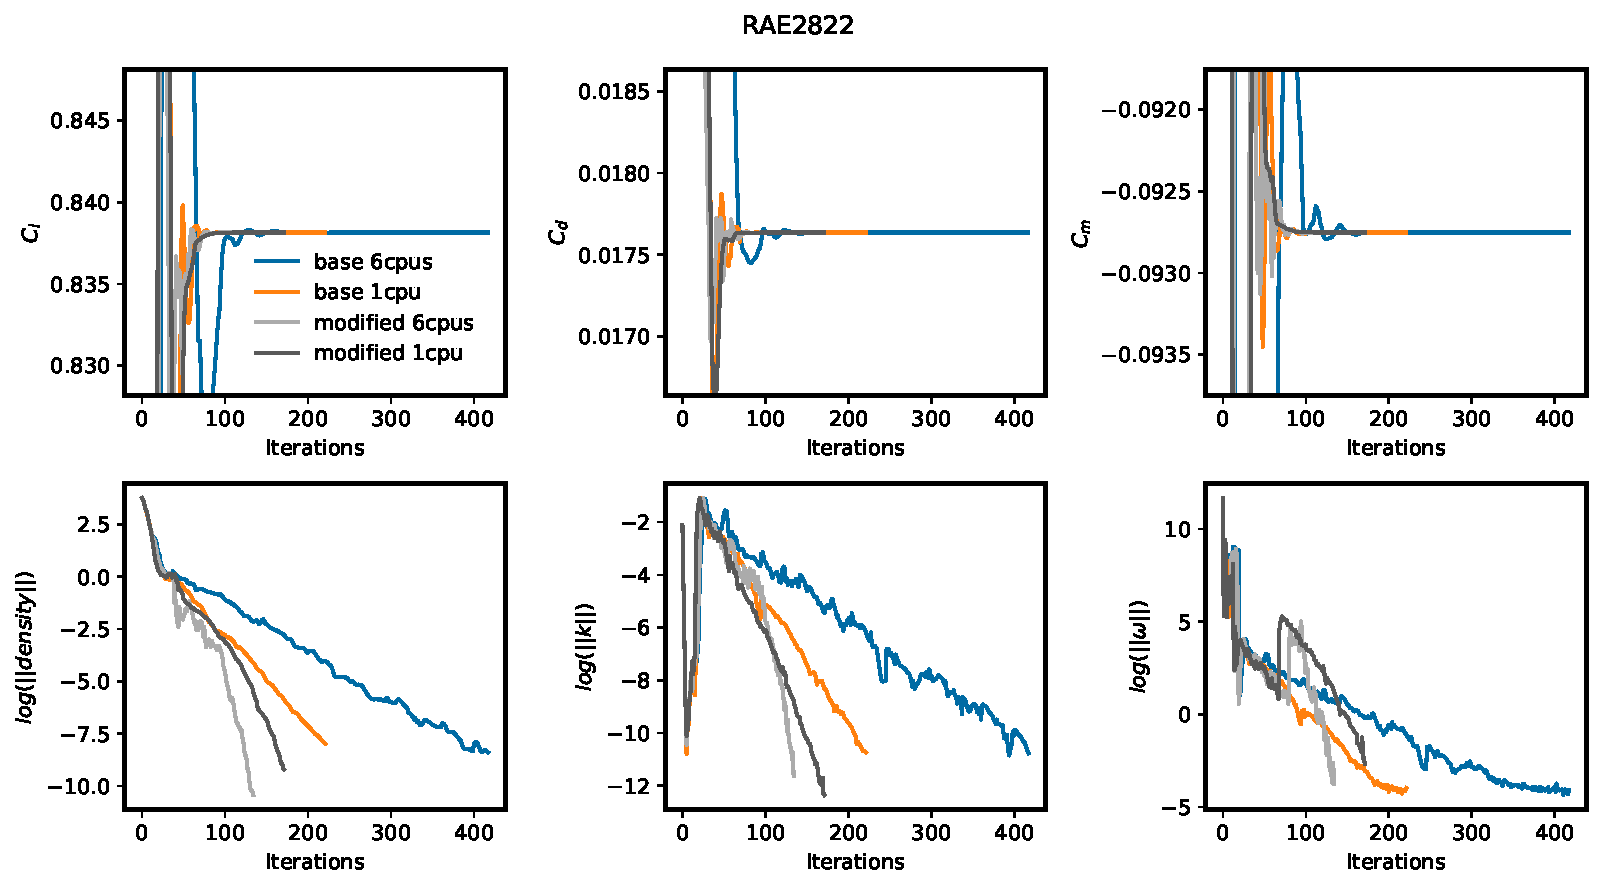
\includegraphics[width=1.0\textwidth]{plots/sc_RAE2822}
    \caption{Convergence history for RAE2822 testcase.}
    \label{fig:sc_RAE2822}
\end{figure}

\noindent First, lets glance ath the baseline. This has also been obtained
using the ANK solver for the flow variables and the DADI solver for the
decoupled turbulence variables. A similar pattern to the NACA
testcase appears: 1 cpu takes only half the iterations of what 6 cpus need.
But, the converged values are the same. When comparing the general line pattern
to the NACA testcase, it appears to be more 'wiggly' here. The author belieaves
this is due to the coarse mesh and transsonic regime. This probably increases
the sensitivity to the CFL number. During convergence, the ANK solver increases
the CFL number based on the current relative convergence. But the high
sensitivity makes the solver unstable and i starts to diverge. Once this is
detected, the CFL number is lowered again. This should be avoidable, but maybe
more tuning or even a change to the CFL-ramping algorithm is needed.

When looking at the modified version, a similar picture to NACA emerges. The
strategy was the same, first use ANK with DADI and once a relative convergence
of 1e-6 is reached, the CSANK solver is enganged which shows almost Newton-type
convergence. Although the contrast is not as big. But it also has to be noted
that that the before mentioned CFL dependence played a role here and some
parameters had to be clipped to increase robustness at the cost of convergence.



% FDPC


\section{SST testcases}

\section{Grid Convergence}

\section{Partial derivatives}

\section{Total derivatives}



    \chapter{Conclusion}
    To conclude, this project has made significant strides in enhancing the SST
turbulence model for optimization purposes within ADflow. The following key
points highlight the project's achievements:

First, the distance to the nearest wall had to be extended for halo cells. This
was necessary in order to get rid of some intermediate MPI communication in the
$F_1$ blending function of SST. It was important to get rid of this
communication as it prevented automatic differentiation.

The implementation of Automatic Differentiation (AD) for the SST turbulence
model was a major milestone. This implementation facilitates the efficient
computation of partial derivatives, which are essential for optimization tasks
in ADflow. But also the regular solvers like \textit{Approximate Netwon-Krylov
(ANK)} and \textit{Newton-Krylov (NK)} profit from this as they now have access
to an AD-preconditioner.

It has been shown that the changes did not change the results when compared to
the legacy implementation of SST. Using testcases from NASA's
\textit{Turbulence Modeling Resource (TMR)}, it has also been shown that the
results obtained mostly agree to reference data. Although there is still some
uncertainty because a different production term for the turbulence had to be
used in order do achieve convergence. It was also not possible to obtain
results for the \textit{flatplate} testcase. The author is confident that a bit
more time would address those shortcomings.

It is even possible to obtain total gradients using the adjoint method when
assembling the state residual matrix using forward routines. The aerodynamic
design variables appear to be correct, although to a relatively low tolerance.
This may be explained through the high non-linearity of SST. It is also
important to note that the geometric design variables seem to be wrong.
Additionally, they appear to depend on the number of cpus used. This most
likely indicates a problem with the extension of the wall distance to halo
cells.

When trying to solve the adjoint system using the reverse\_fast routines, on
may get a number. But it is completely wrong. But the author still considers
this an achievement because ADflow does not simply crash.

In order to maintain the quality and integrity of ADflow, regression test are
used. This project did extended them for the SST turbulence model. But because
the implementation of SST is only at a prototype stage, the tests are as well.

\section{Comparison to Goals}
When looking at the goals stated in the introduction (section \ref{sec:goals}),
most of them have been partially achieved. The following lines take a look at
the goals that were missed or only partially fulfilled.

\begin{enumerate}

    \item[4.] Make sure the partial AD derivatives are correct. 
        \begin{itemize}
            \item This has almost been achieved. Only the backwards mode for
                the forces is wrong. Also, the backwards\_fast mode is not
                correct.
        \end{itemize}

    \item[5.] Get the NK/ANK Solver working.
        \begin{itemize}
            \item Apart from the finite differences pre-conditioner, this has
                been achieved.

            \item The physicality check probably needs some adjustment for
                SST.
        \end{itemize}

    \item[6.] Test and verify the implementation
        \begin{itemize}
            \item This has been partially achieved. It would be great if the
                flatplate testcase would have worked. Also the different
                production terms for SST need to be tested more.
        \end{itemize}

    \item[7.] Get the adjoint Solver working.
        \begin{itemize}
            \item Has been achieved in the sense that it does not crash.
        \end{itemize}

    \item[8.] Test and verify the total gradients.
        \begin{itemize}
            \item This has been partially achieved. The aerodynamic design
                variables appear to be correct when using forward AD for the
                state residual matrix. But the aerodynamic variables are
                slightly off. 

            \item The gradients are completely off when using the
                backwards\_fast routines.
        \end{itemize}
\end{enumerate}

To conclude, SST has now achieved a prototype state where it is almost ready
for optimization. There are still some bugs present, but it is clear where they
are and mostly by what they are caused. The only thing that prevented the
author from fixing them was a lack of time. As such, one has to realize that
getting SST fully working for optimization is a big task. Thus, the outcome of
this project should be considered a success.



\section{Outlook}
This report stated openly and clearly where bugs are and by what they are most
likely caused. As fixing those bugs and getting SST ready for production is
probably the most valuable target of a proceeding project, the steps that come
next should be clear. But still, the following lines list the most prominent
points in random order:

\begin{itemize}
    \item Adapt the physicality check in ANK-turb for SST

    \item Get the finite difference preconditioner working in ANK for SST.
        Maybe only the step size needs to be changed.

    \item Make sure the partials are correctly summed up in the reverse
        routines that exchange the wall distance in halos.

    \item Take a closer look at what is going on with total derivatives
        obtained through complex step. The results have shown that there is a
        slight difference between a step size of $1e-40$ and $1e-200$. This
        should not be the case.
        
    \item Make sure all the gradients are correct when solving the adjoint
        system using the forward AD routines.

    \item Fix the partial backwards\_fast derivatives.

    \item Make sure the gradients are correct when using the backwards\_fast
        routines.

    \item Optimize an airfoil using SST and compare it to results obtained
        using SA.
\end{itemize}



    \listoffigures\clearpage
    \listoftables\clearpage


    \printbibliography

\end{document}
